\documentclass{beamer}

\usetheme{Singapore}
\usecolortheme{rose}

\usepackage[utf8]{inputenc}
\usepackage[vietnamese]{babel}

% Cấu hình table và nhập code
\usepackage{tabu,color,listings}
\definecolor{dkgreen}{rgb}{0,0.6,0}
\definecolor{gray}{rgb}{0.5,0.5,0.5}
\definecolor{mauve}{rgb}{0.58,0,0.82}
\lstset{inputpath=Filecodes}
\lstset{frame=none,
	language=[Sharp]C,
	aboveskip=3mm,
	belowskip=3mm,
	showstringspaces=false,
	columns=flexible,
	basicstyle={\small\ttfamily},
	numbers=none,
	numberstyle=\tiny\color{gray},
	keywordstyle=\color{blue},
	commentstyle=\color{dkgreen},
	stringstyle=\color{mauve},
	breaklines=true,
	breakatwhitespace=true,
	tabsize=3
}

% Sử dụng gói algorithm2e để viết thuật toán
\usepackage{algorithm2e}

% Tham chiếu tài liệu tham khảo
\usepackage[round]{natbib} 
\bibliographystyle{plainnat}

\title{ĐỘ TƯƠNG TỰ HÀNH VI CỦA CHƯƠNG TRÌNH VÀ THỰC NGHIỆM}
\author{Đỗ Đăng Khoa}
\institute{KHMT K19 -- ĐHQN}
\date{Quy Nhơn, 25--08--2017}

\begin{document}

\begin{frame}
  \titlepage
\end{frame}

\begin{frame}
  \frametitle{Nội dung}
  \tableofcontents
\end{frame}

\part{}

\section{Giới thiệu}
\begin{frame}
  \frametitle{Học trực tuyến}
  \begin{minipage}{0.39\linewidth}
    
\includegraphics[width=0.9\linewidth]{images/topMOOC.png}
  \end{minipage}
  \hfill
  \begin{minipage}{0.59\linewidth}
    \begin{itemize}
    \item Một số vấn đề
      \begin{itemize}
      \item Người dạy ít, người học đông
      \item Thời gian nghiên cứu
      \item Đánh giá, xếp hạng      
      \end{itemize}
    \item Giải pháp
      \begin{itemize}
      \item Công cụ hỗ trợ tự động
      	\begin{itemize}
      	\item So sánh hai giải pháp
      	\item Tương đương hay tương tự
      	\item Đánh giá, xếp hạng giải pháp
    	\end{itemize}
      \item Đo được độ tương tự về hành vi giữa hai chương trình
      \end{itemize}
  \end{itemize}

  \end{minipage}
\end{frame}

\begin{frame}
  \frametitle{Một số nghiên cứu liên quan}
  %  Nhớ so sánh với luận văn
  \begin{itemize}
  	\item Xếp hạng tự động
  		\begin{itemize}
  			\item \cite{alur2013automated}
  			\item \cite{singh2013automated}  			
  		\end{itemize}
  	\item Kiểm tra sự tương đương giữa hai chương trình
	  	\begin{itemize}
	  		\item \cite{jackson1994semantic}
	  		\item \cite{jiang2009automatic}
	  	\end{itemize}
  	\item Phát hiện đạo code
  		\begin{itemize}
  			\item \cite{baxter1998clone}
  			\item \cite{komondoor2001using}
  		\end{itemize}
  \end{itemize}

\end{frame}

\begin{frame}
  \frametitle{Dynamic Symbolic Execution}   
  \begin{itemize}
  	\item Ý tưởng chính
  	\begin{itemize}
  	\item Dựa trên kiểu dữ liệu đầu vào
	\item Ghi nhận và phủ định các ràng buộc
  	\item Lặp lại quá trình thực thi
  	\end{itemize}
  \end{itemize}

  \begin{exampleblock}{Cách thức hoạt động}
	\begin{minipage}{0.45\linewidth}
	\lstinputlisting[basicstyle=\small]{test_me.cs}
	\end{minipage}
	\hfill
	\begin{minipage}{0.50\linewidth}
	\begin{itemize}
		\item Lần 1
		\begin{itemize}
			\item Hệ thống $ x = 0 $
			\item Biểu trưng $ x = x_{0} $
			\item Ràng buộc $ x_{0} != 10 $
		\end{itemize}
		\item Lần 2
		\begin{itemize}
			\item Hệ thống $ x = 10 $
			\item Biểu trưng $ x = x_{0} $
			\item Ràng buộc $ x_{0} == 10 $
		\end{itemize}
	\end{itemize}		
	\end{minipage}
  \end{exampleblock}
	
\end{frame}

\section{Sự tương tự về hành vi chương trình}
\begin{frame}
	\frametitle{Hai chương trình tương đương}
	\begin{minipage}[t]{0.48\linewidth}
	\lstinputlisting[basicstyle=\footnotesize]{SwitchCase.cs}
	\end{minipage}
	\hfill
	\begin{minipage}[t]{0.48\linewidth}
	\lstinputlisting[basicstyle=\footnotesize]{IfElse.cs}
	\end{minipage}
	\begin{itemize}
		\item Cùng tham số đầu vào $ x $ kiểu \texttt{int}
		\item Trả về giá trị $ y $ phụ thuộc vào $ x $
		\item Cấu trúc khác nhau
	\end{itemize}
\end{frame}


\begin{frame}
  \frametitle{Thực thi của một chương trình}
  \begin{itemize}
  	\item Cho $P$ là một chương trình
  	\item $I$ là tập hợp các trị đầu vào của $P$
  	\item $O$ là tập hợp các giá trị đầu ra của $P$
  	\item Thực thi chương trình	P là ánh xạ: 
  	\[exec: P \times I \rightarrow O\]
  	\item Với $i \in I$, $o \in O$ thực thi chương trình $P$ trên
  	$i$ ta thu được giá trị đầu ra tương ứng $o = exec(P, i)$.
  \end{itemize}  
\end{frame}


\begin{frame}
  \frametitle{Tương đương về hành vi của 2 chương trình}
  \begin{itemize}
  	\item $P_{1}$ và $P_{2}$ là hai chương trình 
  	\item $I$ miền các giá trị đầu vào
  	\item Thực thi giống nhau trên mọi giá trị đầu vào của $I$ 
  	\item Ký hiệu: \[exec(P_{1}, I) = exec(P_{2}, I).\]
  \end{itemize}
 
\end{frame}


\begin{frame}
  \frametitle{Sự khác biệt hành vi}
  \begin{itemize}
  	\item $P_{1}$ và $P_{2}$ là hai chương trình
  	\item $I$ miền các giá trị đầu vào 
  	\item Thực thi khác nhau trên một vài giá
  	trị đầu vào $i \in I$
  	\item Ký hiệu: \[exec(P_{1}, I) \neq exec(P_{2}, I)\]
  \end{itemize}

\end{frame}


\begin{frame}
  \frametitle{Độ tương tự về hành vi}
  \begin{itemize}
  	\item $P_{1}$ và $P_{2}$ là hai chương trình
  	\item $I$ miền các giá trị đầu vào 
  	\item $I_{s} \subseteq I$ sao cho
  	$exec(P_{1}, I_{s}) = exec(P_{2}, I_{s})$
  	\item $\forall j \in I \setminus I_{s}, exec(P_{1}, j) \neq exec(P_{2},
  	j)$
  	\item Độ tương tự về hành vi giữa $P_1$ và $P_2$ là $|I_s|/|I|$
  \end{itemize}
\end{frame}


\section{Một số phép đo độ tương tự}
\begin{frame}
  \frametitle{Lấy mẫu ngẫu nhiên}
  \begin{itemize}  	
  	\item Lấy ngẫu nhiên một số giá trị trên miền vào \\(\emph{Random
  		Sampling -- RS})
  	\item Tính số lượng giá trị hai chương trình
  	thực thi giống nhau
  	\item Mô tả hình thức:
  	\begin{itemize}
  		\item $P_{1}$ và $P_{2}$ là hai chương trình có cùng miền giá trị đầu
  		vào $I$
  		\item $I_{s}$ là tập con ngẫu nhiên của $I$
  		\item $I_{a}$ là tập con
  		$I_{s}$ sao cho $exec(P_{1}, I_a) = exec(P_{2}, I_a)$
  		\item Và $\forall j \in I_{s} \setminus I_{a}$, thì
  		$exec(P_{1}, j) \neq exec(P_{2}, j)$
  		\item $M_{RS}(P_{1}, P_{2}) = \left|I_{a}\right| \diagup
  		\left|I_{s}\right| $.
  	\end{itemize}
  \end{itemize}
\end{frame}


\begin{frame}
  \frametitle{Thuật toán phép đo RS}
  \begin{algorithm}[H]
  	\KwIn{
  		$P_{1}, P_{2}$ hai chương trình cần đo độ tương tự\; 
  		$I$: Miền giá trị đầu vào của $P_{1}, P_{2}$ \;	  	
  	}  	
	Set $I_{s} = Random(I)$ \;
	Set $I_{a} = \emptyset$\;
  	\For{$i \in I_s$}
  	{  			
		\eIf{$ (exec(P_{1}, i) = exec(P_{2}, i)) $}{
			$I_{a} = I_{a} \cup i$\;
		}{
			Next\;
		}
  	}
	\KwOut{$M_{RS}(P_{1}, P_{2}) = \left|I_{a}\right| \diagup
		\left|I_{s}\right| $.}
  \end{algorithm}
\end{frame}


\begin{frame}
  \frametitle{DSE trên chương trình tham chiếu}
  \begin{itemize}
  	\item Áp dụng DSE trên chương trình tham chiếu
  	\\ (\emph{Single program Symbolic Execution -- SSE})
  	\item Phân tích các câu lệnh chương trình tham chiếu
  	\item Xác định tập dữ liệu thử
  	\item Mô tả hình thức
  	\begin{itemize}
	\item $P_{1}$ và $P_{2}$ là hai chương trình có cùng miền giá trị đầu
	vào $I$
	\item $P_{1}$ là chương trình tham chiếu
	\item $I_{s} = DSE(P_{1})$
	\item $I_{a} \subseteq I_s$ sao cho
	$exec(P_{1}, I_a) = exec(P_{2}, I_a)$
	\item $\forall j \in I_{s} \setminus I_{a}, exec(P_{1}, j) \neq
	exec(P_{2}, j)$
	\item $M_{SSE}(P_{1}, P_{2}) = \left|I_{a}\right| \diagup
	\left|I_{s}\right| $.
  	\end{itemize}
  \end{itemize}
\end{frame}


\begin{frame}
  \frametitle{Thuật toán phép đo SSE}
  \begin{algorithm}[H]
  	\KwIn{
  		$P_{1}, P_{2}:$ hai chương trình cần đo tương tự\; 
  		$P_1$ là chương trình tham chiếu\; 
  		$I$: Miền giá trị đầu vào của $P_{1}, P_{2}$\;	  	
  	}  	
  	Set $I_{s} = DSE(P_{1})$ \;
  	Set $I_{a} = \emptyset$ \;
  	\For{$i \in I_{s}$}
  	{  			
  		\eIf{$ (exec(P_{1}, i) = exec(P_{2}, i)) $}{
  			$I_{a} = I_{a} \cup i$\;
  		}{
  			Next\;
  		}
  	}
  	\KwOut{$M_{SSE}(P_{1}, P_{2}) = \left|I_{a}\right| \diagup
  		\left|I_{s}\right| $.}
  \end{algorithm}
\end{frame}


\begin{frame}
  \frametitle{DSE trên chương trình hợp thành}
  \begin{itemize}
  	\item Xây dựng một chương trình hợp thành kết hợp cả hai
  	\item DSE xác định tập dữ liệu thử trên chương trình hợp thành
  	\item Mô hình hóa chương trình hợp thành:
  	\begin{itemize}
  		\item $P_1$ và $P_2$ là hai chương trình có cùng miền vào $I$
  		\item $P_1$ là chương trình tham chiếu
  		\item $P_c = P_1 \oplus P_2$ có dạng
  		$assert(exec(P_{1}, I) = exec(P_{2}, I))$
  		\item  $assert(\dots)$ là hàm đánh giá biểu thức đúng hay sai
  		\item Ký hiệu $exec(P_c,i) = \top$ để chỉ
  		chương trình hợp thành $P_c$ thỏa hàm đánh giá, cũng có nghĩa là hai
  		chương trình thành phần thực thi giống nhau trên đầu vào $i$.
  	\end{itemize}
  \end{itemize}
\end{frame}


\begin{frame}
  \frametitle{Thuật toán phép đo PSE}
  \begin{algorithm}[H]
  	\KwIn{
  		$P_{1}, P_{2}:$ hai chương trình cần đo tương tự\; 
  		$P_1$ là chương trình tham chiếu\; 
  		$I$: Miền giá trị đầu vào của $P_{1}, P_{2}$\;	
  		$P_{3} = P_1 \oplus P_2$\;  	
  	}  	
  	Set $I_{s} = DSE(P_{3})$ \;
  	Set $I_{a} = \emptyset$ \;
  	\For{$i \in I_{s}$}
  	{  			
  		\eIf{$ (exec(P_{1}, i) = exec(P_{2}, i)) $}{
  			$I_{a} = I_{a} \cup i$\;
  		}{
  			Next\;
  		}
  	}
  	\KwOut{$M_{PSE}(P_{1}, P_{2}) = \left|I_{a}\right| \diagup
  		\left|I_{s}\right| $.}
  \end{algorithm}
\end{frame}


\section{Thực nghiệm}

\begin{frame}
  \frametitle{Nguồn dữ liệu}
  \begin{itemize}
  	\item Trò chơi Code Hunt
  	\begin{itemize}
  		\item 24 câu hỏi
  		\item 250 người sử dụng
  		\item Chương trình do sinh viên viết
  	\end{itemize}
  	\item Do tôi tự xây dựng.
  \end{itemize}
\end{frame}

\begin{frame}
  \frametitle{Các công cụ sử dụng}
  \begin{itemize}
  	\item Microsoft Visual Studio
  	\item Công cụ sinh dữ liệu thử PEX
  	\begin{itemize}
  		\item Sản phẩm của Microsoft
  		\item Dựa trên kỹ thuật DSE
  		\item Tích hợp như một Add-in
  	\end{itemize}
  \end{itemize}
\end{frame}


\begin{frame}
  \frametitle{Kết quả thực nghiệm}
  \centering
  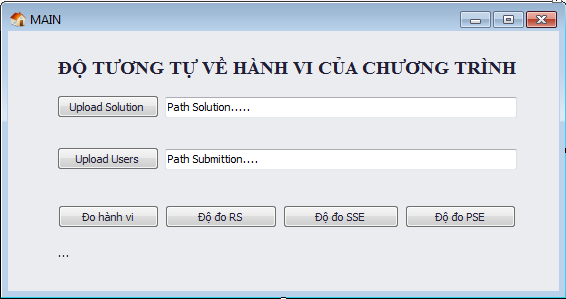
\includegraphics[width=0.6\linewidth]{images/main.png} \\
  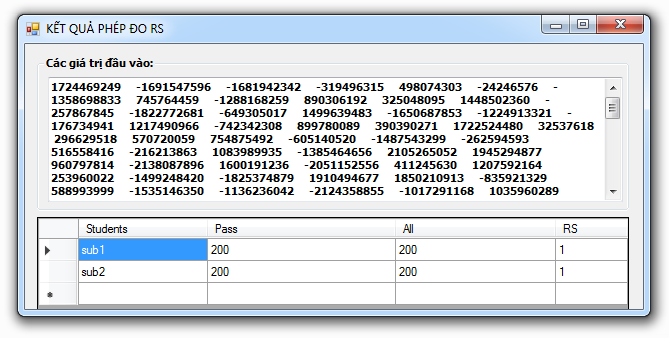
\includegraphics[width=0.6\linewidth]{images/kq_rs.png}
\end{frame}

\begin{frame}
\frametitle{Kết quả thực nghiệm}
\centering
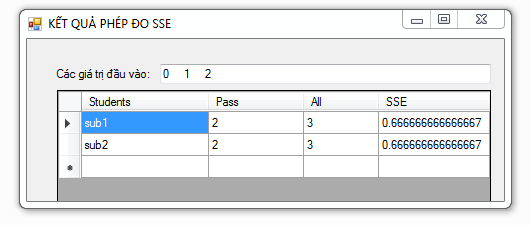
\includegraphics[width=0.8\linewidth]{images/kq_sse.png} \\
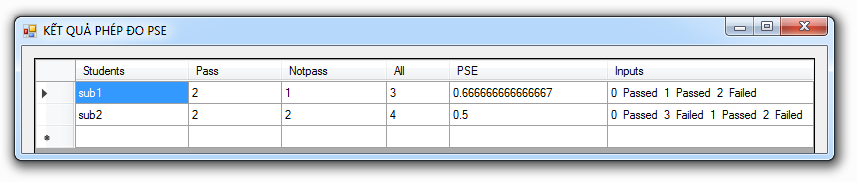
\includegraphics[width=0.8\linewidth]{images/kq_pse.png}
\end{frame}

\begin{frame}
  \frametitle{Kết luận}
  \begin{itemize}
  	\item Hướng phát triển
  	\begin{itemize}
  		\item Cải tiến các phép đo để kết quả được chính xác hơn
  		\item Tích hợp thêm một số ngôn ngữ Java, C++...
  	\end{itemize}
  	\item Khả năng áp dụng
  	\begin{itemize}
  		\item Đánh giá tiến bộ trong lập trình
  		\item Xếp hạng tự động
  		\item Gợi ý giải pháp lập trình
  	\end{itemize}
  \end{itemize}
\end{frame}


\part{}

\begin{frame}
  \begin{center}
    \begin{Huge}
      \textbf{Cảm ơn}
    \end{Huge}
\end{center}

\end{frame}

% Tài liệu tham khảo
\bibliographystyle{plain}
\bibliography{biblio}
\end{document}



%%% Local Variables:
%%% mode: latex
%%% TeX-master: t
%%% End:
